\documentclass[final]{beamer}
\usepackage{biblatex}
\addbibresource{sample.bib}
\usepackage[scale=1]{beamerposter} % Use the beamerposter package for laying out the poster
\usepackage{graphicx}
\usepackage{array}
\usepackage{tabu}
\usepackage[utf8]{inputenc}
\usepackage{subcaption}
\usepackage{listings}
\usepackage{verbatim}




\usetheme{confposter} % Use the confposter theme supplied with this template

\setbeamercolor{block title}{fg=ngreen,bg=white} % Colors of the block titles
\setbeamercolor{block body}{fg=black,bg=white} % Colors of the body of blocks
\setbeamercolor{block alerted title}{fg=white,bg=dgreen!70} % Colors of the highlighted block titles
\setbeamercolor{block alerted body}{fg=black,bg=dblue!10} % Colors of the body of highlighted blocks

\newlength{\sepwid}
\newlength{\onecolwid}
\newlength{\twocolwid}
\newlength{\threecolwid}
\setlength{\paperwidth}{48in} % A0 width: 46.8in
\setlength{\paperheight}{36in} % A0 height: 33.1in
\setlength{\sepwid}{0.024\paperwidth} % Separation width (white space) between columns
\setlength{\onecolwid}{0.22\paperwidth} % Width of one column
\setlength{\twocolwid}{0.464\paperwidth} % Width of two columns
\setlength{\threecolwid}{0.708\paperwidth} % Width of three columns
\setlength{\topmargin}{-0.5in} % Reduce the top margin size
%-----------------------------------------------------------

\usepackage{graphicx}  % Required for including images

\usepackage{booktabs} % Top and bottom rules for tables

\title{Dialogue generation with transformers} % Poster title

\author{{\huge Shivangi Khandekar, Josep Rubió Piqué}} % Author(s)

\institute{{\huge UAB, Natural Language Processing}} % Institution(s)

\begin{document}

\addtobeamertemplate{block end}{}{\vspace*{2ex}} % White space under blocks
\addtobeamertemplate{block alerted end}{}{\vspace*{2ex}} % White space under highlighted (alert) blocks

\setlength{\belowcaptionskip}{2ex} % White space under figures
\setlength\belowdisplayshortskip{2ex} % White space under equations

\begin{frame}[t] % The whole poster is enclosed in one beamer frame

\begin{columns}[t] % The whole poster consists of three major columns, the second of which is split into two columns twice - the [t] option aligns each column's content to the top

\begin{column}{\sepwid}\end{column} % Empty spacer column

\begin{column}{\onecolwid} % The first column


\begin{alertblock}{Abstract}
	\begin{itemize}
	\item Try to create an AI agent giving meaningful responses on dialogues.
    \item Use transformer and self-attention architecture instead of RNN.
    \item Trained with OpenSubtitles dateset.
	\end{itemize}
\end{alertblock}

\begin{block}{Dataset}

OpenSubtitles is an open corpus with movies subtitles in different languages.\\
\vspace{10mm}
The dataset used to train the agent are the english subtitles from OpenSubtitles:
	\begin{itemize} 
	\item $\sim140$M utterances
	\item Dirty dataset. Metadata from the movie, comments not related to dialogues, ...
    \item Scripts from PolyAI used to clean the dataset
    \item Trained with just the previous sentence in the context.
	\end{itemize}\\[1\baselineskip]
	
 \texttt{\{}
 
 \texttt{"file\_id": "lines-aaa",}
 
 \texttt{"context": "They always do.", }
 
 \texttt{"response": "Hmm, but they don't.", }
 
\texttt{"context/0": "He will.",}

\texttt{"context/1": "What then?",}
  
\texttt{...}

\texttt{\}}
\end{block}

%{"file_id": "lines-aaa", "context": "They always do.", "response": "Hmm, but they don't.", "context/0": "He will.", "context/1": "What then?",

\begin{block}{Attention is all you need}
	\begin{itemize} 
	\item Traditional \textbf{Encoder-Decoder} architecture without RNN or convolutional networks
	\item Based on attention concept. Learning of Query (\textbf{Q}), Key (\textbf{K}) and Value(\textbf{V}) matrices
    \item \textbf{Stacked transformers} for encoder and decoder and \textbf{multi head} attention to \textit{attend to different information}
	\item \textbf{Positional encoding} to give relative position information to tokens. In the paper a $\sin$ function added to embedding
	\item For decoder an extra \textbf{masked attention} layer is used to learn the language model. It cannot look forward so it masks attention for not generated tokens
	\end{itemize}

\end{block}

\end{column} % End of the first column

\begin{column}{\sepwid}\end{column} % Empty spacer column

\begin{column}{\twocolwid} % Begin a column which is two columns wide (column 2)

\begin{columns}[t,totalwidth=\twocolwid] % Split up the two columns wide column

\begin{column}{\onecolwid}\vspace{-.6in} % The first column within column 2 (column 2.1)

\begin{block}{Transformer Architecture}
    \begin{figure}
    %\centering
    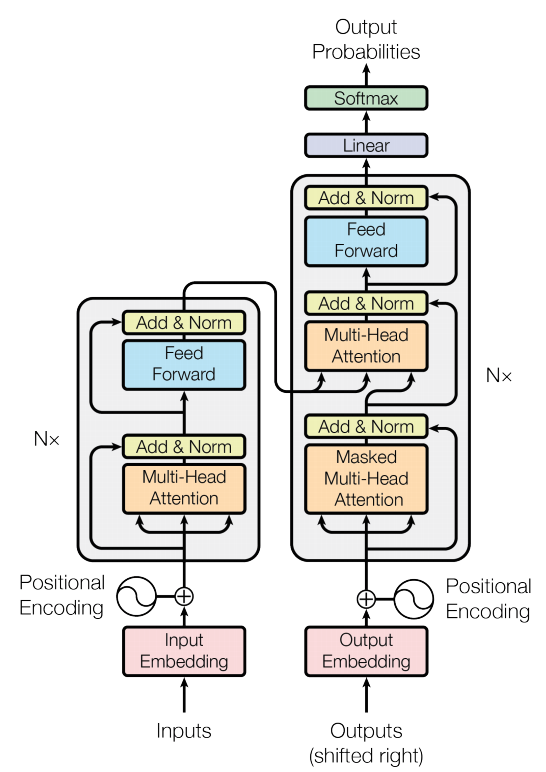
\includegraphics[clip,scale=0.88]{transformer.png}
    \caption{Transformer architecture}
    \end{figure}

\begin{figure}
\centering
\begin{subfigure}{.5\textwidth}
  \centering
  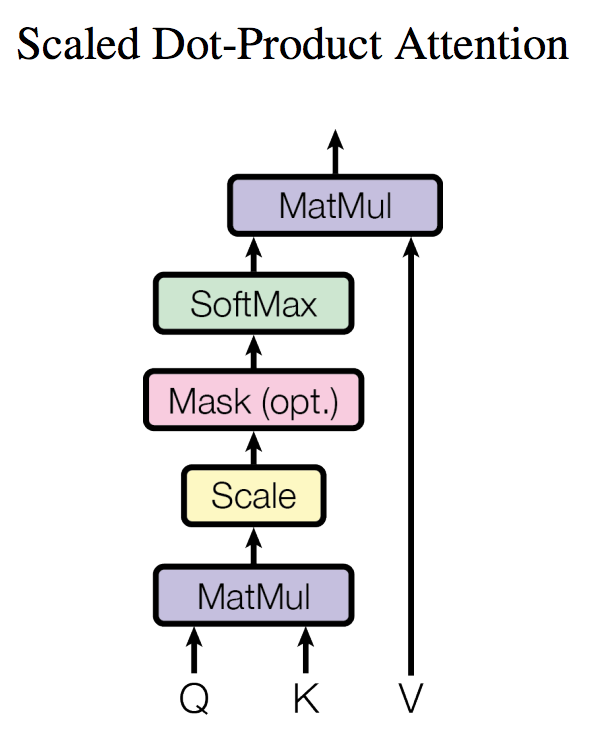
\includegraphics[scale=0.98]{dotproduct.png}
  \caption{Scaled dot product attention}
  \label{fig:sub1}
\end{subfigure}%
\begin{subfigure}{.5\textwidth}
  \centering
  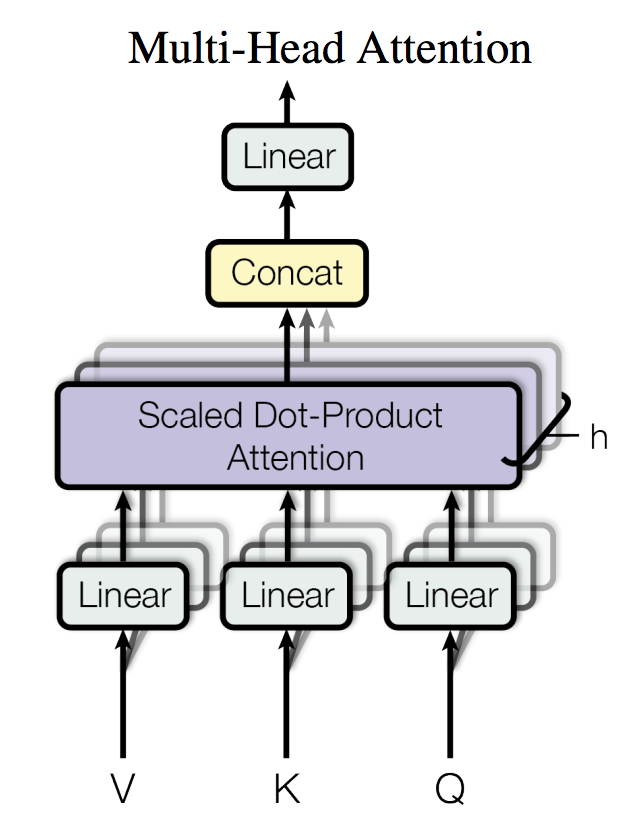
\includegraphics[scale=0.98]{multihead.png}
  \caption{Multi-Head attention}
  \label{fig:sub2}
\end{subfigure}
\caption{Attention}
\label{fig:test}
\end{figure}

    \begin{figure}
    %\centering
    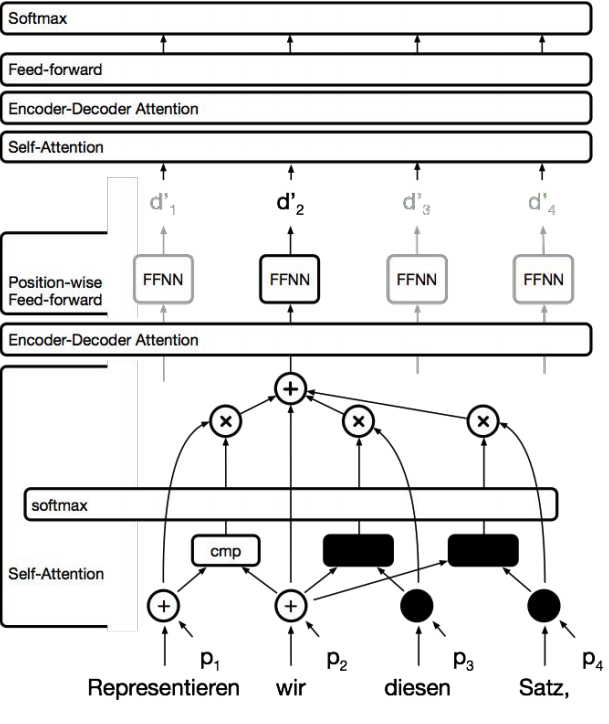
\includegraphics[clip,scale=0.78]{transformer3.png}
    \caption{Decoder architecture}
    \end{figure}

\end{block}

\end{column} % End of column 2.1
\begin{column}{\onecolwid}\vspace{-.6in} % The second column within column 2 (column 2.2)

\begin{block}{Transformer implementation and outcomes}

Implementation based on \textit{Transformer model for language understanding} from TensorFlow. 

\begin{itemize} 
	\item Subword tokenizer from TensorFlow Dataset library
	\item Token embedding using Keras embedding layer
	\item 4 encoder layers
	\item 4 decoder layers
	\item Sublayers and embedding outputs of size 128
	\item Feed Forward inner layer of size 512
	\item 8 attention heads
	\end{itemize}

\begin{alertblock}{Small train dataset}

Trained with 78.000 utterances and 20 EPOCHS. 2 hr in a personal computer:

\begin{itemize} 
	\item \textbf{Context:} \textit{Hello I am John.}
	\item \textbf{Predicted response:} \textit{I'm not gonna be a doctor.}
\end{itemize}

\begin{itemize} 
	\item \textbf{Context:} \textit{Who are you?}
	\item \textbf{Predicted response:} \textit{I am a bit much.}
\end{itemize}

\begin{itemize} 
	\item \textbf{Context:} \textit{I want to eat a sandwich}
	\item \textbf{Predicted response:} \textit{I want to be a doctor!}
\end{itemize}\\
\end{alertblock}

\begin{alertblock}{Big train dataset}

Trained with $\sim2$M utterances and 10 EPOCHS. 10 hr in the cloud and a GPU:

\begin{itemize} 
	\item \textbf{Context:} \textit{My name is John.}
	\item \textbf{Predicted response:} \textit{I'm sorry........ Achi. Achi......}
\end{itemize}

\begin{itemize} 
	\item \textbf{Context:} \textit{Good morning.}
	\item \textbf{Predicted response:} \textit{Where are you???????????????????}
\end{itemize}

\begin{itemize} 
	\item \textbf{Context:} \textit{I am in my car}
	\item \textbf{Predicted response:} \textit{What the fuck are you talking about???????????}
\end{itemize}

\begin{itemize} 
	\item \textbf{Context:} \textit{I am going to the hospital}
	\item \textbf{Predicted response:} \textit{What the fuck are you talking about???????????}
\end{itemize}
\end{alertblock}

\end{block}

\end{column} % End of column 2.2

\end{columns} % End of the split of column 2 - any content after this will now take up 2 columns width

\begin{columns}[t,totalwidth=\twocolwid] % Split up the two columns wide 

\end{columns} % End of the split of column 2

\end{column} % End of the second column

\begin{column}{\sepwid}\end{column} % Empty spacer column

\begin{column}{\onecolwid} % The third column

\begin{alertblock}{Big train dataset}

Trained with the recommended architecture from the paper. The same but \textbf{6} encoder and decoder layers, outputs of size \textbf{512} and FF inner layer of size \textbf{2048}. The response is the same for all contexts.\\

\vspace{10mm}

Trained with $\sim2$M utterances and 3 EPOCHS. 9 hr in the cloud and a GPU:

\begin{itemize} 
	\item \textbf{Context:} \textit{My name is John.}
	\item \textbf{Context:} \textit{Good morning.}
	\item \textbf{Context:} \textit{I am in my car}
	\item \textbf{Context:} \textit{I am going to the hospital}
\end{itemize}

\begin{itemize} 
	\item \textbf{Predicted response:} \textit{I don't know what you're talking about. about.with.with.with.about.with.with.with.with.}
\end{itemize}

\end{alertblock}

\begin{block}{Evaluation}
The main way to evaluate the results in dialogue generation is with human judgement, comparing the result of the agent with other responses generated from other agents. I cold not evaluate my results this way.
\end{block}

\begin{block}{Conclusion \& Future Work}

\begin{itemize} 
	\item It seems the results keep getting worst as it gains more information.
	\item Underfitting with less information?
	\item It seems the model converges to give dull responses, which could make sense from a dialogue prospective if a similar sentence to the context does not exist in the dataset
	\item The model learns a "language model" that creates responses grammatically correct fast but it does not give meaningful responses in the dialogue. 
	\item Hard to deal with big datasets for time and space constraints.
	\item Training the agent with a big dataset with the recommended architecture properly.
\end{itemize}

\end{block}

\begin{block}{References}
\begin{itemize}
\item \textit{Vaswani, Attention is all you need}
\item Tensorflow Transformer model for language understanding \url{https://www.tensorflow.org/tutorials/text/transformer}
\item OpenSubtitles corpus \url{http://opus.nlpl.eu/OpenSubtitles-v2018.php}
\item Poly AI \textit{Conversational Datasets} \url{https://github.com/PolyAI-LDN/conversational-datasets}

\end{itemize}
\end{block}

\end{column} % End of the third column

\end{columns} % End of all the columns in the poster

\end{frame} % End of the enclosing frame

\end{document}
